
\documentclass[PICOReport.tex]{subfiles}

\begin{document}

%\vskip 10pt

%%%% Old introduction
%The angular power spectra of sky-based $Q$ and $U$ polarization Stokes parameters are commonly recast in terms of curl-free $E$ mode and gradient-free $B$ mode patterns. $E$ modes are generated by either scalar fluctuations, such as density perturbations in the early Universe or by tensor perturbations, such as gravitational waves. $B$ modes are only generated through tensor perturbations. The Probe of Inflation and Cosmic Origins (PICO) is an imaging polarimeter designed to survey the entire sky at frequencies between 21 and 800 GHz with a polarization sensitivity that is 57 or 82 times that of the \planck\ mission for the PICO baseline and \ac{CBE} configurations, respectively. 

%PICO's science reach is extraordinarily broad. The mission requirements, which define our baseline design, flow down from a smaller set of science objectives (SO) listed in Table~\ref{tab:STM}. This baseline gives rise to a mission that will reach a much broader set of science targets, as described in this report. 
%%PICO's data will enrich and complement other astrophysical surveys in the next decade. 
%The \ac{CBE} is our current estimate for the actual performance of the mission. \comor{where are we outlining the assumptions for the CBE}. 

%Fluctuations of the space-time metric during the epoch of inflation, near the Planck time, have generated gravitational waves that embed a unique $B$-mode signature on the polarization of the CMB. A detection of this \ac{IGW} signal "would be a watershed discovery", a quote from the 2010 decadal panel report~\citep{blandford2010}, as it would be our first signal from the epoch of quantum gravity at the beginning of the Universe. The signal would also give strong clues about the nature of inflation, as the $B$-mode signal is proportional to the energy scale of inflation through a parameter commonly labeled $r$, the tensor-to-scalar ratio. The combination of data from \planck\ and the BICEP/Keck Array give the strongest constraint to date $r<0.06\,\, (95\%)$~\citep{2018arXiv181005216A}.
%%This limit has already ruled out several models for the inflaton potential~\citep{planck2018inflation}. 
%%An intense campaign is ongoing by sub-orbital instruments to reduce the limit on $r$ and perhaps detect the 
%%inflationary B-mode signal.  
%But the measurements have also revealed that emission within our own galaxy is a source of confusion that must be separated with high fidelity before definitive discovery, or stronger upper limits, can be claimed~\citep{whichplanck}. For the levels of $r\lesssim 0.001$ as targeted in the next decade, see SO1 (Table~\ref{tab:STM}), an exquisite separation of Galactic emissions is required, particularly for measurements at the largest angular scales. For these levels of $r$ it will also be necessary to control systematic uncertainties at unprecedented levels. \comor{Improved measurements of the spectral index of primordial fluctuations $n_{s}$, a consequence of PICO's sensitivity and angular resolution, will give the strongest constraints yet on specific models of inflation (SO2). }
%
% 

The Probe of Inflation and Cosmic Origins (PICO) is an imaging polarimeter designed to survey the entire sky at 21 frequencies between 21 and 800 GHz with a polarization sensitivity that is 57 or 82 times that of the \planck\ mission for the PICO baseline and current best estimate (\ac{CBE}) configurations, respectively. 

The mission requirements, which define our baseline design, flow down from a small set of key science objectives listed in Table~\ref{tab:STM}. As outlined in this report, this baseline gives rise to a mission that will reach an extraordinarily broad set of science targets, ranging from inflation, to constraints on fundamental particles and fields, to cosmic structure formation and galactic science.
%PICO's data will enrich and complement other astrophysical surveys in the next decade. 
%The \ac{CBE} is our current estimate for the actual performance of the mission. \comor{where are we outlining the assumptions for the CBE}. 

According to inflation, quantum fluctuations in the space-time metric created a background of gravitational waves that imprint a unique signature on the polarization of the CMB. A detection of this \ac{IGW} signal "would be a watershed discovery", a quote from the 2010 decadal panel report~\citep{blandford2010}. It would be the first observational evidence for quantum gravity. The signal would also give important clues about the nature of inflation, in particular the energy scale at which it occurred. The strength of the signal is commonly parameterized by a parameter commonly labeled $r$, the tensor-to-scalar ratio. The combination of data from \planck\ and the BICEP/Keck Array give the strongest constraint to date $r<0.06\,\, (95\%)$~\citep{2018arXiv181005216A}.

Emission within our own galaxy is a source of confusion that must be separated with high fidelity before definitive discovery, or stronger upper limits, can be claimed~\citep{2016A&A...586A.133P}. For the levels of $r$ targeted in the next decade, PICO has both the frequency coverage and sensitivity to measure and separate sources of foreground confusion and is thus poised to detect or place unprecedented constraints on the physics of inflation. \comor{Its measurements of the spectral index of primordial fluctuations will give the strongest constraints yet on specific models of inflation. }

%PICO has the frequency coverage and sensitivity to measure and separate sources of foreground confusion and is thus poised to detect or place unprecedented constraints on the physics of inflation. \comor{Its measurements of the spectral index of primordial fluctuations will give the strongest constraints yet on specific models of inflation. }

A few hundred million years after the Big Bang, the neutral hydrogen gas permeating the Universe was reionized by photons emitted by the first luminous sources to have formed.  The nature of these sources (e.g., star-forming galaxies or high-redshift quasars) and the exact history of this epoch are key missing links in our understanding of structure formation.  Various measurements, including \planck 's measurement of the optical depth to reionization $\tau = 0.054 \pm 0.007$, have indicated that reionization concluded by $z \approx 6$, but its onset at higher redshift is poorly constrained. PICO will yield a breakthrough in this context via a cosmic-variance-limited\footnote{The cosmic variance limit is the statistical limit arising from observing a single universe.} measurement of $\tau$, with $\sigma(\tau)=0.002$, which can only be directly measured in large-scale CMB polarization fluctuations (this is SO5).  The only proven method to date for measuring this signal, which requires exquisite control of systematics and foreground contamination, is a space-based platform. 

\begin{figure}[!thb]
\centering
\hspace{-0.15in}
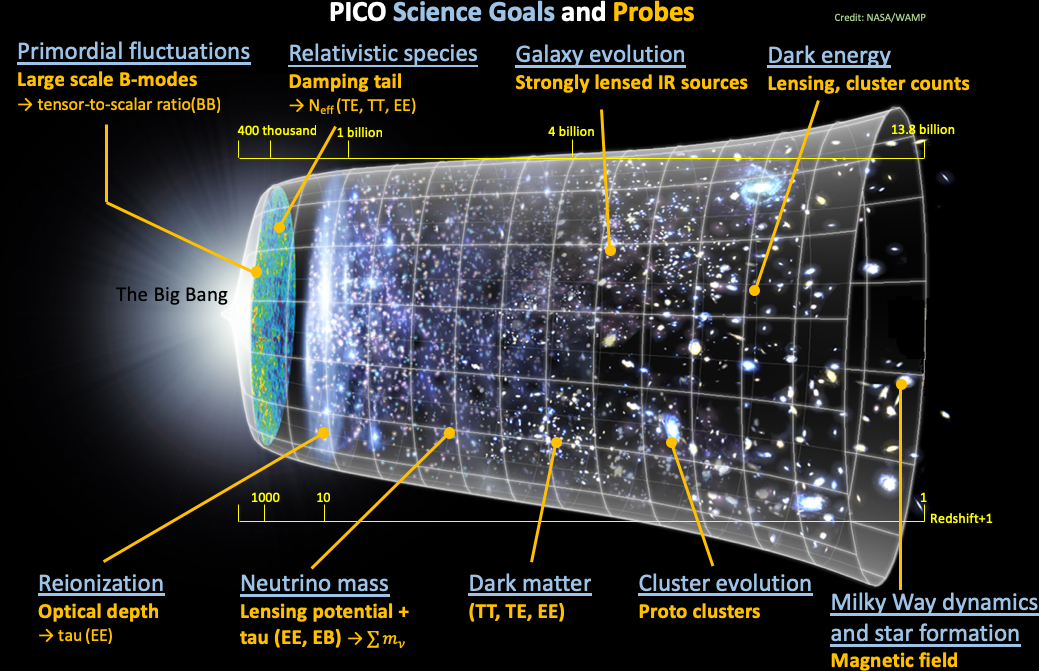
\includegraphics[width=5.5in]{images/PICO_science goals and probes.png}
\hspace{-0.15in}
\caption{Caption}
\label{fig:PICOsci_probes}
\end{figure}

Lensing of the CMB photons by structures as they traverse the Universe provides a projected map of all the matter in the universe from the epoch of decoupling until today.  The non-zero mass of neutrinos affects the clustering of matter and thus can be inferred from maps of the projected matter distribution. The quantity that can specifically be inferred is the sum of the neutrino masses.  The current constraint from the combination of \planck\ and large-scale structure data is $\sum m_{\nu} < 0.12$ eV (95\%).  This is approaching the minimum summed mass allowed in the inverted neutrino hierarchy of $\approx 0.1$ eV and is within a factor of two of the minimal mass allowed in the normal hierarchy of $\approx 0.06$ eV.  A detection thus appears imminent.  However, the precision of determining the neutrino mass scale, using the CMB or {\it any} other cosmological probe, is limited by knowledge of $\tau$, due to the strong degeneracy between $\tau$ and the amplitude of matter fluctuations.  PICO's map of the projected matter with \ac{SNR} exceeding 500 -- a result of its low noise and high angular resolution -- {\it and} its own cosmic-variance-limited measurement of $\tau$ will give a $4\sigma$ detection of $\sum m_{\nu}$ in the normal hierarchy, rising to $\sim7\sigma$ for the inverted hierarchy; see SO3. 

%A direct measurement of $\tau$ via the large-scale $E$-mode polarization signal is thus required in order to break this degeneracy and enable a detection of the sum of the neutrino masses.  The current uncertainty from \planck, $\sigma(\tau) \approx 0.007$, will already limit neutrino mass constraints from cosmological experiments in the next five years; in order to go beyond this, a cosmic-variance-limited measurement with $\sigma(\tau) = 0.002$ must be achieved.  Due to its multifrequency capabilities, all-sky coverage, and excellent control of systematics, PICO is the ideal experiment to achieve this goal.

The CMB offers a unique window into the thermal history of the universe, from the time of reheating through today.  It is during these eras that the matter and radiation that fill the universe were produced and evolved to form the structures observed at low redshifts.  Measurements of the CMB on small angular scales are sensitive to the many components that make up the universe including the baryons, cosmic neutrinos, dark matter, and a wide variety of particles motived by extensions of the Standard Model.  The Standard Model of particle physics posits three neutrino families, but it also allows for additional light, relativistic particles, if they existed early enough during the evolution of the Universe.   We count the total number light particles thermalized in the early universe using $\Neff$. Light particles thermalized in the early universe leave a universal contribution to $\Neff$ that is sensitive to the freeze-out temperature and the spin of the particle.  The current \planck\ measurement of $\Neff = 2.99 \pm 0.17 \,\, (1\sigma)$ is sensitive to particles thermalized after the QCD phase transitions. PICO's measurement with $\sigma(\Neff)=0.03$ (SO4), enabled by low noise levels, high resolution, and full sky coverage, will reach back to times when the temperature of the universe was orders of magnitude hotter than we have probed today, and a period that is still largely unexplored.   
These same experimental features are advantageous not only for $\Neff$ but for any new physics with signatures on the CMB. Of particular interest is the nature of dark matter and its interactions. PICO will place constraints that are more than on order of magnitude stronger than \planck\ for a dark matter particle of MeV mass range, which can not be probed by direct detection experiments. PICO will thus reveal important clues to the nature of the fundamental laws and our cosmic origins. 

%As the history of the universe prior to a few seconds is still largely unexplored, PICO will reveal important clues to the nature of the fundamental laws and our cosmic origins. 

% Such a measurement would shed light on the history of the universe at those very early times and will address important questions about the particles and forces in the Standard Model and Beyond.  The history of the universe prior to a few seconds is still largely unexplored observationally and PICO will reveal important clues to the nature of the fundamental laws and our cosmic origins.

%The current measurement of $\Neff = 2.99 \pm 0.17$ from Planck is sensitive to particles thermalized after the QCD phase transitions.  Reaching much earlier time is possible with PICO because of much lower noise levels in polarization.  Larger sky coverage further improves the statistics and compensates for the lower resolution compared to ground based measurements.  These features are advantageous not only for $\Neff$ for any new physics present in the primary CMB and/or lensing potential.  Of particular interest is the nature of dark matter and its interactions, which can be manifest itself in any or all of these probes, depending on the details physics of the dark sector. 


%Measuring CMB polarization at small angular scales will bring many of the questions about the universe into sharp focus.  Of particular interest is the projected improvements to the number of relativistic species, $\Neff$.  Light particles thermalized in the early universe leave a universal contribution to $\Neff$ that is sensitive to the freeze-out temperature and then spin of the particle.  A mission like PICO holds the promise to reach back to times when then temperature of the universe was orders of magnitude hotter than we have probe today.  Such a measurement would shed light on the history of the universe at those very early times and can address important questions about the particles and forces in the Standard Model and Beyond.

%\comor{the paragraph below covers a lot of ground, but the anticipated impact is not clear. do we want to mention cluster counts? the impact of source counts? Gianfranco thinks pico is unique, but this is not clear.  Need to say what PICO will do for these topics - Nick, thoughts? NB: I gave this a shot}  

Secondary anisotropy in the CMB\footnote{Secondary anisotropy arises from sources other than primordial density and \ac{IGW} fluctuations} provide a wealth of information on the growth and evolution of structure in our universe. CMB lensing, the thermal and kinematic \ac{SZ} effects, and extragalactic point sources all contribute significantly to the CMB intensity fluctuations on small angular scales (note that lensing is also present in polarization fluctuations). Immense progress in mapping these sources is enabled by PICO's depth, broad frequency coverage, and relatively high resolution. The all-sky, projected mass map reconstructed from CMB lensing that PICO will provide can be correlated with tracers of large-scale structure to tomographically probe the growth of structure at unprecedented \ac{SNR} levels. The thermal SZ effect provides a map of the integrated free electron pressure along the line of sight, and the peaks of this map trace the locations of all galaxy clusters in the universe. PICO will find all the massive, virialized, galaxy clusters at any redshift.  The epoch of reionization imprints information in the statistical moments of the kinematic SZ signal. The combination of these kSZ statistical moments with the cosmic variance limited $\tau$ measurementfrom PICO will provide tight constriants on the global properties of the sources responsible for reionization the universe.
%Combining thermal and kinematic SZ measurements of galaxies will yield important information about the thermodynamics of galaxy formation, as well as the precise location of the ``missing baryons''. 

Our understanding of magnetic fields is rooted in observations of the very local universe: the Milky Way and nearby galaxies. Magnetic fields are observed to be a foremost agent of the Milky Way's ecology. Understanding magnetic field is crucial for making progress on some exciting issues in the astrophysics of galaxies: the dynamics and energetics of the multiphase interstellar medium, the efficiency of star formation, the acceleration and propagation of cosmic rays and the 
impact of feedback on galaxy evolution.Through its detailed high resolution polarization measurements of galactic dust emission PICO will produce an unprecedented data set mapping galactic magnetic fields and providing answers to these questions (SO6 and 8). 

Magnetic fields are not only critical for understanding the dynamics and evolution of galaxies. The very origin of magnetic fields in galaxies, and their possible evolution from primordial, early universe cosmic magnetic fields is a topic of intense debate. PICO is poised to provide definitive answer as to whether early universe magnetic fields could provide the seeds for most current galaxies. 

The magnetized ISM in the Solar Neighborhood presents a challenge for the investigation of cosmological signals. Cosmological signals of interest, such as CMB B-mode polarization, CMB spectral distortions, and 21cm line emission from the cosmic dawn and the reionization epoch are obscured by galactic dust and synchrotron emission that can be orders of magnitude brighter. PICOs detailed mapping of these signals will strongly constrain the physical properties of the ISM and thus models of dust grain composition, temperature, and emissivities (SO7). 

The PICO deep and high resolution maps will yield a treasure trove of point source that will be mined for years. The mission will provide a full sky catalog of tens of thousands of extragalactic millimeter and sub-millimeter point sources, which are beacons for active galactic nuclei (in the radio) and dust emission from vigorously star-forming galaxies at $z \sim 2$ and earlier (in the far-IR). 

%Cosmic magnetism is an outstanding puzzle of fundamental importance to astrophysics. Magnetic fields are ubiquitous, and their evolution is critically interwoven with the dynamics of the universe. Hence, it is crucial to understand their origin and the dynamo processes that must have amplified weak  primordial seed fields and maintained their strength across cosmic time \citep{Brandenburg2005}. 

%\comor{need to add words about galactic science} 

\end{document}

%\begin{figure}[!htb]
%\centering
%
\includegraphics[width=4cm]{images/example}
%\caption{example}
%\label{fig:im_4}
%\end{figure}
